% !TeX root = ../main.tex

\chapter{Using This Template}\label{chap:template}

This chapter is a working example of everything the template can typeset.
Delete it once you have copied out the pieces you need --- nothing else depends
on it.

\section{Sections and Cross-References}

Chapters, sections, and subsections are numbered automatically. Give anything
you want to point at a \verb|\label|, then refer to it with \verb|\ref|, and
the number stays correct however much you reorder the document later.

\subsection{A Subsection}

Subsections nest one level deeper and still appear in the table of contents.
Going deeper than \verb|\subsubsection| is possible but rarely reads well.

Footnotes work as usual.\footnote{Keep them short. A footnote that runs longer
than the paragraph anchoring it usually belongs in the body or an appendix.}

\section{Mathematics}

Inline mathematics such as $E = mc^2$ sits in the run of text. Displayed
equations are numbered and can be referenced like anything else:
%
\begin{equation}
\label{eq:example}
\bar{x} = \frac{1}{n} \sum_{i=1}^{n} x_i .
\end{equation}
%
Equation~\eqref{eq:example} defines the sample mean.

% wherelist 是這個模板自訂的環境（定義在 environments.tex），
% 用來在公式後面列出符號說明，「where」會自動印出來。
% wherelist is defined in environments.tex. It prints the word "where" for you
% and aligns the symbol column automatically.
The custom \texttt{wherelist} environment explains the symbols directly beneath
an equation, in the style most engineering and science journals expect:
%
\begin{equation}
\label{eq:variance}
s^2 = \frac{1}{n-1} \sum_{i=1}^{n} \left( x_i - \bar{x} \right)^2 ,
\end{equation}
\begin{wherelist}
  \item[$s^2$] is the sample variance;
  \item[$n$] is the number of observations;
  \item[$x_i$] is the $i$-th observation;
  \item[$\bar{x}$] is the sample mean defined in Equation~\eqref{eq:example}.
\end{wherelist}

\section{Figures}

A single figure floats to a convenient place on the page. The optional argument
of \verb|\caption| is the short form that appears in the List of Figures, which
keeps a long explanatory caption from swamping the front matter.

\begin{figure}[htbp]
  \centering
  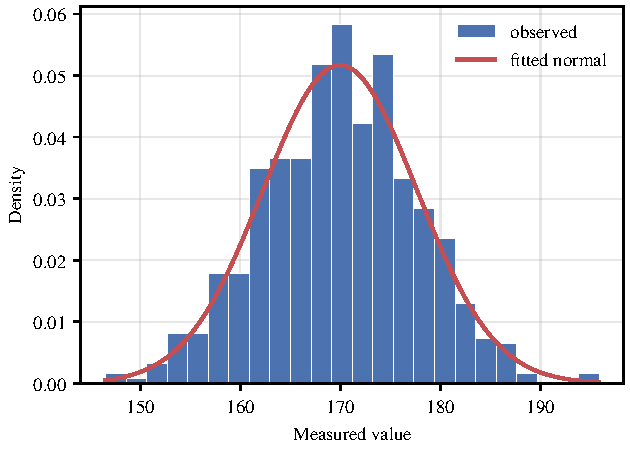
\includegraphics[width=0.7\linewidth]{figures/example-histogram.pdf}
  \caption[Distribution of a measured quantity]{Distribution of a measured
  quantity, with the fitted normal density drawn on top. Give the reader
  everything needed to interpret the figure without hunting through the body
  text: what was measured, how many observations, and what the curve is.}
  \label{fig:histogram}
\end{figure}

Figure~\ref{fig:histogram} is referenced by label, so its number survives being
moved to another chapter.

Several related panels belong in one float, each with its own sub-caption and
label:

\begin{figure}[htbp]
  \centering
  \begin{subfigure}{0.48\linewidth}
    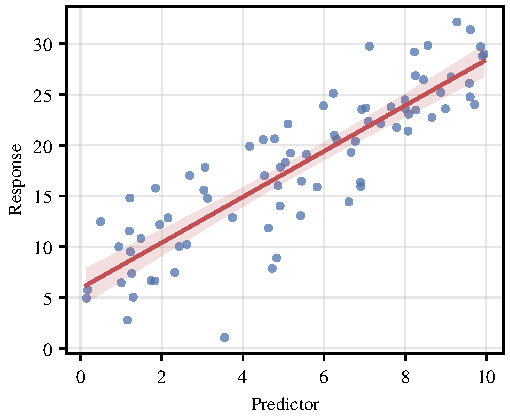
\includegraphics[width=\linewidth]{figures/example-scatter.pdf}
    \caption{Linear fit with a 95\% confidence band}
    \label{fig:scatter}
  \end{subfigure}
  \hfill
  \begin{subfigure}{0.48\linewidth}
    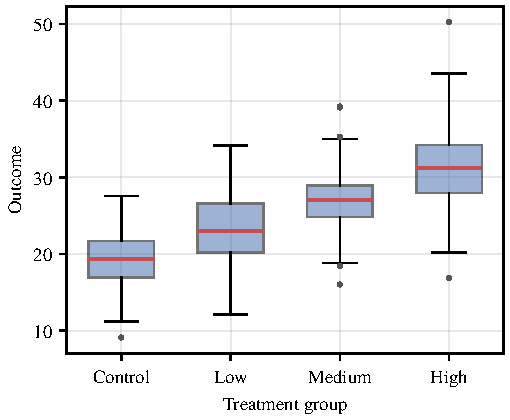
\includegraphics[width=\linewidth]{figures/example-boxplot.pdf}
    \caption{Distribution by treatment group}
    \label{fig:boxplot}
  \end{subfigure}

  \vspace{1em}

  \begin{subfigure}{0.48\linewidth}
    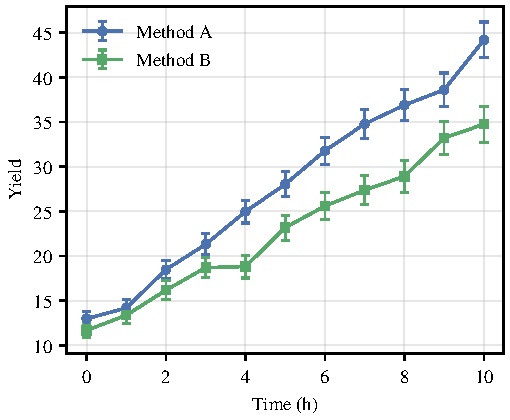
\includegraphics[width=\linewidth]{figures/example-errorbar.pdf}
    \caption{Two methods over time, with standard errors}
    \label{fig:errorbar}
  \end{subfigure}
  \caption[Three common ways of presenting a comparison]{Three common ways of
  presenting a comparison. Sub-figures are referenced individually, as in
  Figure~\ref{fig:scatter}, or as a group, as in Figure~\ref{fig:panels}.}
  \label{fig:panels}
\end{figure}

Vector PDFs keep their quality at any zoom level and are what plotting
libraries should be asked to emit. Bitmap formats are a last resort, and photos
belong in PNG or JPEG at a resolution high enough to survive printing.

\section{Tables}

\texttt{booktabs} gives tables the horizontal rules journals expect. Vertical
rules and double rules are deliberately hard to draw with it, because they make
tables harder to read.

\begin{table}[htbp]
  \centering
  \caption{Summary statistics by treatment group}
  \label{tab:summary}
  \begin{tabular}{lrrr}
    \toprule
    Group   & $n$ & Mean & Std.\ dev. \\
    \midrule
    Control &  90 & 19.8 & 4.1 \\
    Low     &  90 & 23.2 & 5.0 \\
    Medium  &  90 & 26.9 & 4.4 \\
    High    &  90 & 31.6 & 5.9 \\
    \bottomrule
  \end{tabular}
\end{table}

Table~\ref{tab:summary} sits above its data by convention: table captions go on
top, figure captions underneath. Note that the caption comes before the
tabular material in the source, and that a table wider than the text block
should be rotated or moved to an appendix rather than shrunk until it is
illegible.

\section{Source Code}

\texttt{minted} colours code through Pygments, which needs the compiler to run
with \verb|-shell-escape|. Overleaf enables this by default, and the local
build in this repository passes the flag for you.

\begin{minted}[fontsize=\small]{python}
def sample_variance(values):
    """Return the unbiased sample variance of a sequence of numbers."""
    n = len(values)
    if n < 2:
        raise ValueError("variance needs at least two observations")
    mean = sum(values) / n
    return sum((value - mean) ** 2 for value in values) / (n - 1)
\end{minted}

Short fragments read better inline: \mintinline{python}{sum(values) / n}.

\section{Citations}

\texttt{biblatex} manages citations, and \texttt{biber} processes the
bibliography. In \texttt{main.tex}, the configured
\mbox{\texttt{numeric-comp}} style compresses consecutive numbers into a range.

A plain citation looks like this~\cite{warren1890}. Several at once collapse
automatically~\cite{said1978,fisher1936,vaswani2017}. \texttt{biblatex} also
offers \verb|\parencite| for a parenthesised form~\parencite{surgeongeneral1964}
and \verb|\textcite| for one that reads as part of the sentence:
\textcite{geertz1973} makes this point directly.

The bibliography in \texttt{back/references.bib} carries one real, published
example of every entry type \texttt{biblatex} supports, so you can copy the
closest match rather than guessing which fields a type requires.
